\chapter{Cooper-Paare und Supraleitung\label{chapter:supraleitung}}
\lhead{Cooper-Paare und Supraleitung}
\begin{refsection}
\chapterauthor{Simon Kuster und Nicola Ochsenbein}

\newcommand{\marrow}[5]{%
    \fmfcmd{style_def marrow#1
    expr p = drawarrow subpath (1/4, 3/4) of p shifted 6 #2 withpen pencircle scaled 0.4;
    label.#3(btex #4 etex, point 0.5 of p shifted 6 #2);
    enddef;}
    \fmf{marrow#1,tension=0}{#5}}
\begin{center}
\begin{fmffile}{supraleitung/phonon}
\begin{fmfgraph*}(100,60)
\fmfleftn{i}{2}
\fmfrightn{o}{2}
\fmflabel{$\vec k'-\vec q$}{i1}
\fmflabel{$\vec k'$}{i2}
\fmflabel{$\vec k+\vec q$}{o1}
\fmflabel{$\vec k$}{o2}
\fmf{fermion}{i2,v1,i1}
\fmf{fermion}{o2,v2,o1}
\fmf{zigzag,label=$\vec q$}{v1,v2}
\fmfdot{v1,v2}
\marrow{c}{up}{top}{}{v1,v2}
\end{fmfgraph*}
\qquad
\qquad
\qquad
\begin{fmfgraph*}(100,60)
\fmfleftn{i}{2}
\fmfrightn{o}{2}
\fmflabel{$\vec k'+\vec q$}{i1}
\fmflabel{$\vec k'$}{i2}
\fmflabel{$\vec k-\vec q$}{o1}
\fmflabel{$\vec k$}{o2}
\fmf{fermion}{i2,v1,i1}
\fmf{fermion}{o2,v2,o1}
\fmf{zigzag,label=$-\vec q$}{v1,v2}
\fmfdot{v1,v2}
\marrow{c}{up}{top}{}{v2,v1}
\end{fmfgraph*}
\end{fmffile}
\end{center}

Entstehung von Cooper-Paaren und Supraleitung nach Feynman
%\caption{Entstehung von Cooper-Paaren und Supraleitung nach Feynman
%\label{supraleitung:FeynmanDiagram1}}
\cite{supraleitung:feynman}.


\newpage
%----------------------------Einleitung------------------------
\section{Einleitung}
\rhead{Einleitung}
In diesem Kapitel m"ochten wir die Grundlagen f"ur die Supraleitung erarbeiten. Ausgehend von der bekannten coulombschen Wechelwirkung zwischen Elektronen, wollen wir verstehen wie und aus welchem Grund sich Elektronen zu Paaren binden, sogenannte Cooper-Paare. Dazu m"ussen wir zuerst den Effekt der Elektron-Elektron Wechselwirkung verstehen. Aufbauend k"onnen wir dann erkl"aren, welches die energetisch g"unstigsten und somit auch wahrscheindlichsten Konstellationen sind, unterwelchen sich die Elektronen zu Paaren binden.
%TODO Einleitung so ok, der l"anger?

%----------------------------Elektron-Elektron Wechselwirkung------------------------
\section{Elektron-Elektron Wechselwirkung\label{supraleitung:elektronelektronwecheslwirkung}}
\rhead{Elektron-Elektron Wechselwirkung}
Es gibt neben der coulombschen Wechselwirkung zwischen den Elektronen noch mehr Wechselwirkungen. Zum einen gibt es eine Elektronen-Gitter Wechselwirkung. Diese ist f"ur die Betrachung der Cooper-Paare aber nicht relevant. Sie wird deshalb nachfolgend nicht ber"ucksichtigt. Zum anderen gibt es eine Elektron-Elektron Wechselwirkung "uber die sogenannten Phononen. Wie diese Wechselwirkung im Allgemeinen funktioniert und was diese Phononen sind wird nachfolgend erl"autert.
\\
In Abbildung \ref{supraleitung:Gitter1} betrachten wir einen Ausschnitt der Gitterstruktur eines K"orpers. Fliegt nun ein Elektron in dieses Gitter hinein, so wird das Gitter durch das elektrische Feld des Elektrons deformiert. Das Elektron "andert seine Flugbahn. Dargestellt ist dies in Abbildung \ref{supraleitung:Gitter2}. Das deformierte Gitter bewegt sich nun weiter als Schwingung. In Abbildung \ref{supraleitung:Gitter3} ist diese Schwingung dargestellt und mit $q$ bezeichnet. Wenn nun ein weiteres Elektron ins Gitter fliegt, so wird dieses von der Schwingung im Gitter beeinflusst, ersichtlich in Abbilung \ref{supraleitung:Gitter4}. Die Schwingung im Gitter wird wieder vernichtet und das zweite Elektron ver"andert ebenfalls seine Flugbahn. Es wurde also ein Impuls vom Elektron $k'$ zum Elektron $k$ "uber das Gitter transportiert. 
\\
Die Schwingng $q$ welche vom Elektron $k'$ zum Elektron $k$ transportiert wurde entspricht einem harmonischen Oszillator. Das Bedeuted, dass die m"oglichen Frequenzen, und die damit die enthaltenen Energieniveaus, quantisiert sind. Wenn diese Energie quantisiert ist, kann man die Energie auch als Teilchen betrachten. Diese neu eingef"uhrten Teilchen werden Phononen genannt.
Um die Darstellung der Wechselwirkung zu vereifachen, zeichnen wir nun die Gitterschwingung als zickzack Vektor zwischen Elektron $k'$ und $k$. Diese Darstellung Feynman ist in Abbildung \ref{supraleitung:FeynmanDiagram1} ersichtlich.%TODO hier sollte auf das Feynmandiagramm verwiesen werden. (wie?)
%Kann das verhalten der Bilder so beeinflusst werden, dass sie wenigstens im gleichen unterkapitel angezeigt werden? (momentan ist die Darstellung der Bilder "uber so viele Seiten nicht geeignet.
\begin{figure}
\centering
\includegraphics[width=0.4\textwidth]{supraleitung/gitter-1.pdf} %Bild Ungestoertes Gitter
\caption{Ungest"ortes Gitter
\label{supraleitung:Gitter1}}
\end{figure}
\begin{figure}
\centering
\includegraphics[width=0.4\textwidth]{supraleitung/gitter-2.pdf} %Bild Gitter mit Elektron1
\caption{Elektron fliegt ins Gitter und st"ort dieses
\label{supraleitung:Gitter2}}
\end{figure}
\begin{figure}
\centering
\includegraphics[width=0.4\textwidth]{supraleitung/gitter-3.pdf} %Bild Gitter mit Stoerung
\caption{Gitter mit Schwingung q
\label{supraleitung:Gitter3}}
\end{figure}
\begin{figure}
\centering
\includegraphics[width=0.4\textwidth]{supraleitung/gitter-4.pdf} %Bild Gitter mit Elektron2
\caption{Elektron fliegt ins Gitter und wird beeinflusst
\label{supraleitung:Gitter4}}
\end{figure}
\\
Diese Wechselwirkung zwischen den Elektronen kann mathematisch beschrieben werden. F"ur die mathematische Betrachtung beginnen wir da wo wir einen Anhaltspunkt haben, also beim Phonon.
\\
Wir haben gesehen, dass das Phonon quantisiert ist. F"ur dieses gibt es also Auf- und Absteigeoperatoren. Wenn wir das Phonon $a$ nennen und die Energie $q$ haben, ergibt sich der Aufsteigoperator $a^+_q$ und den Absteigeoperator $a_q$. Da die vom Phonon aufgenommene Energie quantisiert ist, so muss das Elektron qunatisierte Energie aufnehmen und abgeben. Dies bedeuted, dass das Elektron Auf- und Absteigeoperatoren haben. Wir nennen die Elektronen nun $c$ mit der Wellenzahl $k$. Daraus folgt, dass der Aufsteigoperator f"ur das Elektron $c^+_k$ und der Absteigeoperator $c_k$ sind.
Wir f"uhren nun noch einen Anfangszustand $|a\rangle$, einen Endzustand $\langle e|$ und einen Zwischenzustand $|z_1\rangle$ ein. Der Vorgang der Wechselwirkung zwischen den Elektronen kann nun so beschrieben werden (ohne Energiebetrachtung):
\begin{equation}
\langle e|c^+_{k+q} c_k a_q |z_1\rangle\langle z_1| c^+_{k'-q} c_{k'} a^+_q |a\rangle
\label{supraleitung:WechelwirkungOE}
\end{equation}
Zu beachten ist nun, dass die Leserichtung von rechts nach links ist. Es wird also vom Anfangszustand aus ein Phonon $a$ mit der Energie $q$ erzeugt, ein Elektron $c$ mit der Wellenzahl $k'$ vernichtet und ein Elektron $c$ mit der Wellenzahl $k'+q$ erzeugt, um zum Zwischenzustand $z_1$ zu gelangen.
Von diesem Zwischenzustand aus geht es weiter, indem man das Phonon $a_q$ wieder vernichtet, das Elektron $c_k$ vernichtet und ein Elektron $c^+_{k+q}$ erzeugt.
\\
Als n"achstes m"ussen wir die Energiebetrachtung einf"ugen. Daf"ur F"uhren wir eine materialabh"angige Konstante $M_q$ ein und erg"anzen die Wechselwirkung mit dem Nenner aus der St"orungstheorie.
Um die gesammte Wechselwirkung zu erhalten summieren wir "uber alle $k$,$k'$ und $q$. Die Wechselwirkung erg"anzen wir zudem um einen zweiten Term der die umgekehrte Reihenfolge enth"alt. Dieer f"uhrt dazu, dass wir sp"ater weitere vereifachungen durchf"uhren k"onnen. Da wir aber nun die Wechselwirkung doppelt z"ahlen (wir summieren ja bereits "uber alles) teilen wir noch durch $2$.
\\
\begin{equation}
\frac{1}{2}
\sum \limits_{kk'q} |M_q|^2
\left\{
\frac
{\langle e|c^+_{k+q} c_k a_q |z_1\rangle\langle z_1| c^+_{k'-q} c_{k'} a^+_q |a\rangle }
{E(k')-E(k'-q)-\hbar\omega_q}
+
\frac
{\langle e|c^+_{k'-q} c_{k'} a_{-q}|z_1\rangle\langle z_1| c^+_{k+q} c_k a^+_{-q} |a\rangle }
{E(k)-E(k+q)-\hbar\omega_q}
\right\}
\label{supraleitung:WechelwirkungME}
\end{equation}
\\
Da $E(k')-E(k'-q)-\hbar\omega_q = E(k)-E(k+q)-\hbar\omega_q$ ist, ersetzen wir in der Formel den ersten mit dem zweiten.
\\
Zus"atzlich k"urzen wir die Phononen heraus und packen alles ausser der reinen Wechselwirkung in einen Koeffitienten $V_{kk'q}$. Somit erhalten wir zwei Formeln:
\begin{equation}
\frac{1}{2}
\sum \limits_{kk'q} 
\langle e|V_{kk'q}c^+_{k+q}c^+_{k'-q}c_{k'}c_k|a \rangle
\label{supraleitung:WechelwirkungKurz}
\end{equation}
und
\begin{equation}
V_{kk'q} = - |M_q|^2 \left\{\frac{1}{\hbar\omega_q+(E(k+q)-E(k))}
+
\frac{1}{\hbar\omega_q-(E(k+q)-E(k))}
\right\}
\label{supraleitung:WechelwirkungVkk'q}
\end{equation}
Das Vorzeichn von $V_{kk'q}$ entscheidet nun dar"uber, ob die Wechselwirkung anziehend oder abstossend ist.
\begin{equation}
\frac
{2|M_q|^2\hbar\omega_q}
{(E(k+q)-E(k))^2-(\hbar\omega_q)^2}
\label{supraleitung:Wechelwirkung_Vkk'q_Kurz}
\end{equation}
%TODO nun muss die Formel 81.2 eingefuehrt werden -> Nenner noch nachvollziehbar beschreiben.
%danach richtung 81.4 weiterziehen
\\
\\
\\
Weitere Formeln:
\\
\begin{equation}
V_{kk'q} =
\frac
{2|M_q|^2\hbar\omega_q}
{(E(k+q)-E(k))^2-(\hbar\omega_q)^2}
\label{supraleitung:WechelwirkungEnd}
\end{equation}
\\
\\
TODO: Formeln noch einbauen und erkl"aren

%----------------------------Hinzufuegen von Elektronen zu der Fermikugel------------------------
\section{Hinzuf"ugen von Elektronen zu der Fermikugel}
\rhead{Hinzuf"ugen von Elektronen zu der Fermikugel}
Angenommen, solch eine Elektron-Elektron Wechselwirkung, wie im Kapitel \ref{supraleitung:elektronelektronwecheslwirkung} beschrieben kommt zustand. Doch welche Bedingungen m"ussen erf"ullt sein?
\\
Unser Ziel wird nun sein, zwei Elektronen energetisch m"oglichst g"unstig zur Fermikugel hinzuzuf"ugen. Dazu ben"otigen wir die theoretischen Grundlagen zur Fermikugel welche im Kapitel \ref{chapter:festkoerper} behandelt sind.
\\
In welcher Form k"onnen zwei Elektronen am energetisch g"unstigsten zu der Fermikugel hinzugef"ugt werden? Mit dieser Frage wollen wir uns nun besch"aftigen.
\\
\\
Die Wechselwirkung zwischen den Elektronen besteht einerseits aus der altbekannten Coulombsche Wechselwirkung~(\ref{supraleitung:Coulombsches Gesetz}) und der neu eingef"uhrten Elektronen-Elektronen Wechselwirkung. Welcher dieser Kr"afte "uberwiegt, entscheidet die St"arke der Elektron-Phononen-Kopplung.
\\
\begin{equation}
F=\frac{Q_A\cdot Q_B}{4\pi\epsilon r^2}
\label{supraleitung:Coulombsches Gesetz}
\end{equation}
\\
Um diese neue Wechselwirkung zu betrachten gehen wir von einem idealisierten Falls aus, 
%TODO elektronengas, kgek"uhlter k"orper
. 
Wir betrachten die Fermikugel in der $k$-Ebene, in welcher alle inneren Zust"ande besetzt sind, alle "ausseren Zust"ande seien frei. Zu diesem System werden nun zwei Elektronen $(k_1,E(k_1))$ und $(k_2,E(k_2))$ hinzugef"ugt. Wir beschr"anken uns auf die Wechselwirkungen in welchen keine Energie an das Atomgitter abgegeben wird. Zudem beschr"anken wird die zul"assige Wechselwirkung zwischen den Elektronen auf die Energie eines Phonons.

\begin{equation}
|E(k+q)-E(k)|\le\hbar\omega_q
\label{supraleitung:Phonon Energie}
\end{equation}

Wellenfunktion
Die Wellenfunktion des Elektronenpaares wir durch die Anwendung zweier Erzeugnisoperatoren auf den Grundzustand $|G\rangle$ der gef"ullten Fermikugel aufgebaut, indem wir "uber alle m"oglichen $k_1$ und $k_2$ $(|k_i| \ge k_f)$ und "uber die Elektronenspins summieren.

\begin{equation}
\Psi_{12}=\sum \limits_{k_1k_2\sigma_1\sigma_2} a_{\sigma_1\sigma_2}(k_1,k_2)c^+_{k_1\sigma_1}c^+_{k_2\sigma_2}|G\rangle
\label{supraleitung:Wellenfunktion ganz Allgemein}
\end{equation}

Um einen Zustand mit definiertem Gesamtimpuls zu erhalten, f"uhren wir die Summation unter der Nebenbedingung $K=k_1+k_2=const$ aus.

%TODO Hier weiter machen
Das n"achste Ziel wird nun sein diese Wechselwirkungsenergie zu berechnen. Sie ist umso gr"osser, je mehr Summationsglieder zu obigen Wellenfunktion beitragen. W"ahlt man $K=0$ erzielt man die gr"osste Wechselwirkungsenergie. Um diesen "Uberlegungsschritt nachzuvollziehen betrachten wir die Abbildung \ref{supraleitung:kRaum_1}...
\\
% Visualisierung der besten K-Vektors
% Visualisierung 1
\begin{figure}	
\centering
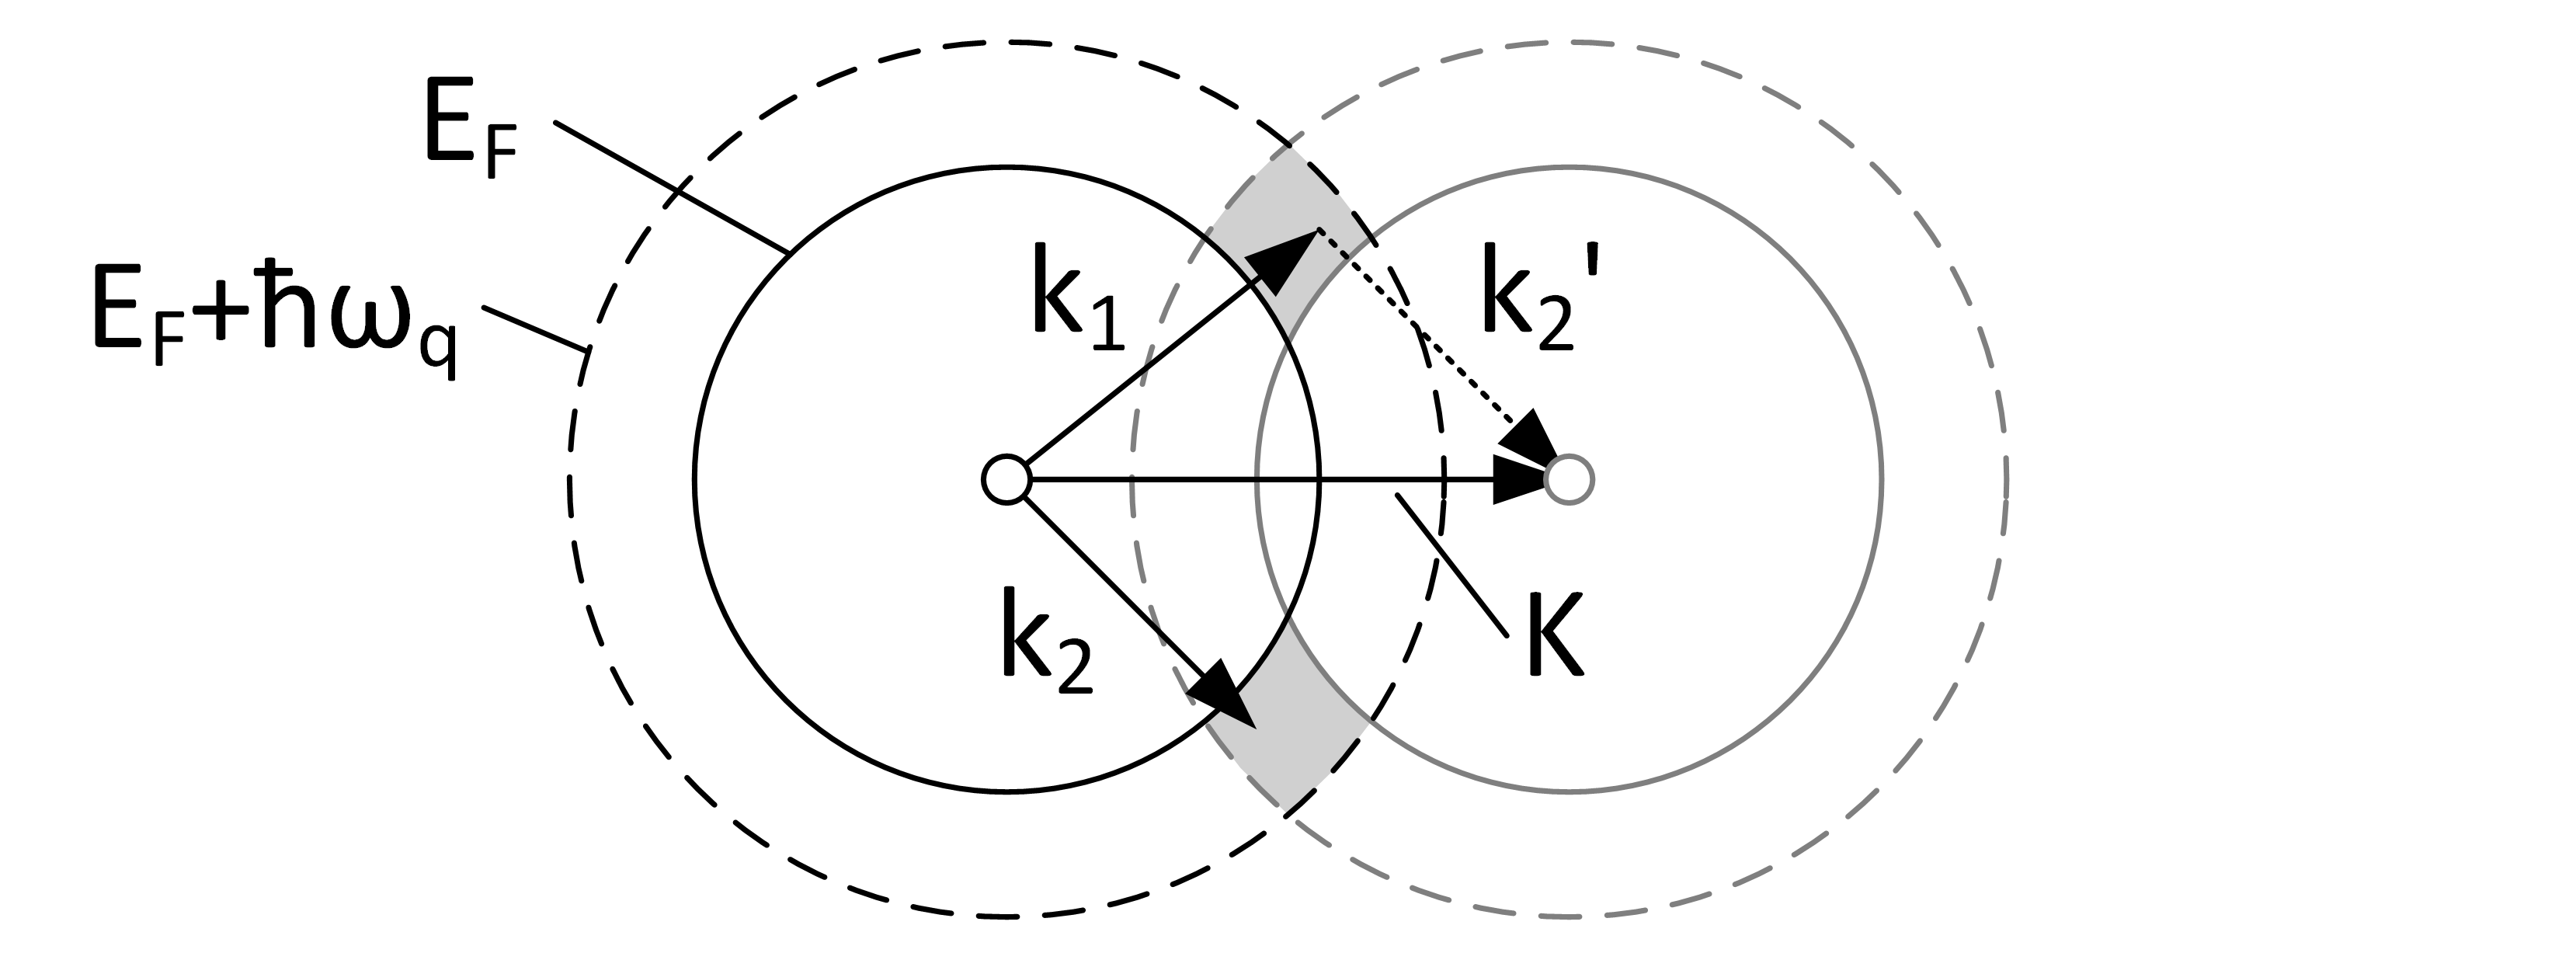
\includegraphics[width=0.6\textwidth]{supraleitung/kGraphic_05.png} %K gr"osser 0, kleiner Ef+hwq, mit Fl"achenmarkierung
\caption{Visualisierung im k-Raum
\label{supraleitung:kRaum_1}}
\end{figure}
% Visualisierung 2
\begin{figure}	
\centering
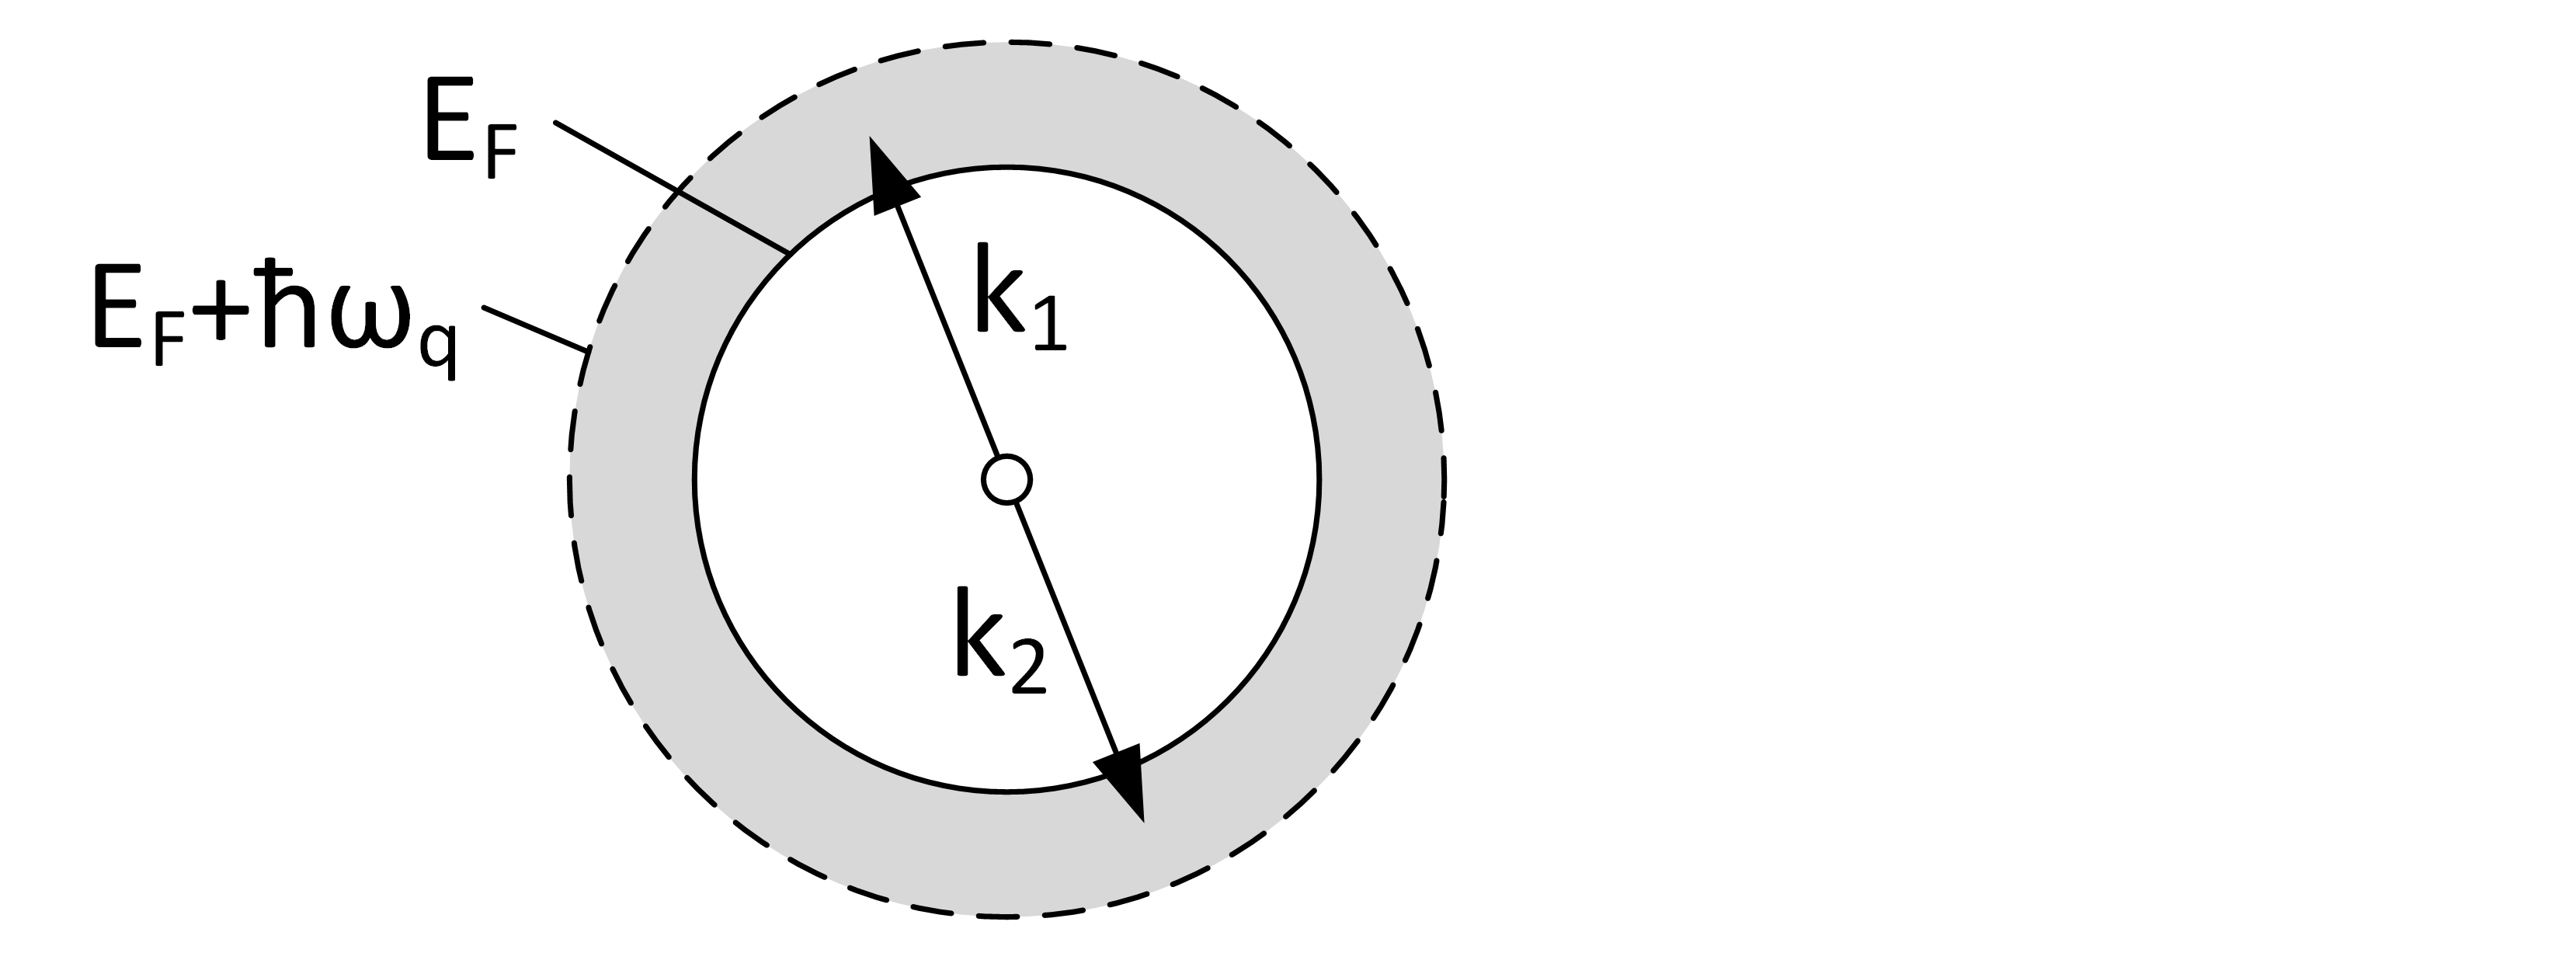
\includegraphics[width=0.6\textwidth]{supraleitung/kGraphic_09.png} %K gleich 0, mit Fl"achenmarkierung
\caption{Maximale Anzahl M"oglichkeiten um $k_1$, $k_2$ zu w"ahlen
\label{supraleitung:kRaum_2}}
\end{figure}

Eine Wechselwirkung zwischen den Elektronen soll nur dann bestehen, wenn sich ihre Zust"ande ausserhalb der Fermikugel mit den Energie $(E_F \le E(k_i) \le E_F+\hbar\omega_p)$ befinden. Da $K=k_1+k_2$ gilt ergeben sich bei $K>0$ im k-Raum folgende grau eingef"arbte Bereich. Die Fl"ache kann maximiert werden indem $K=0$ gesetzt wird. F"ur die folgenden Berechnungen werden wir uns auf diesen Fall beschr"anken.
Zus"atzlich nehmen wir an, dass die Elektronenspins antiparallel sind. Hierzu kann die "Uberlegung mit dem entstehenden magnetischen Feld herbeigezogen werden. W"aren der Elektronenspin parallel w"urden sich die entstehenden magnetischen Felder abstossen. Wobei hingegen bei antiparallelem Elektronenspin die Wechselwirkungsenergie durch die anziehenden magnetischen Felder verst"arkt wird.
Somit ergibt sich die neue Wellenfunktion

\[
\Psi_{12}=\sum \limits_{k} a(k)c^+_{k}c^+_{-k}|G\rangle
\]

$k$ ordnen wir zugleich „Spin aufw"arts“ und $–k$ f"ur „Spin abw"arts“ zu.
Der g"unstigste Prozess ist also wenn die Elektronen entgegengesetzte Wellenzahlvektoren $(k_1 = -k_2)$ und entgegengesetzten Spin $(\sigma_1 = -\sigma_2)$ aufweisen.
\\
%\section{Elektronenverhalten in einem Festk"orper}
%\rhead{Elektronenverhalten in einem Festk"orper}
\\
\printbibliography[heading=subbibliography]
\end{refsection}

